\section{Modelling the Game}
\label{sec:model}

% what this section talks about
%   - graph of objects and relations
%   - what each model object represents and is
%   - difficulties developing the model
%   - model: sector, game, entity, ship, plan, goal, ship action, ship class, ship configuration, weapon, system, weapon slot, system slot, fleet, Formation, client state
% what is a game model
% early on
% 

The model that makes up the game consists of the internal representation of the various game entities, such as ships and planets, as well as the business logic that is used to manage and control them and the relationships between them. During the alpha phase, this model was rather simple as it only existed to store the locations of the entities. As development progressed, it grew in complexity and feature completeness. Currently there are two sets of models: one for the fleets of ships, and the other for the map of planets and spacelanes.\sidenote{Spacelanes are connections between some planets that allow ships travelling along or nearby them to move more quickly. See Section~\ref{sec:pathfinding} for complete details.} This section will describe and discuss these models and the reasonings behind their design.

\subsection{Sectors and Planets}

\begin{margintable}
    \begin{tabular}{p{4em} p{11em}}
    \toprule
    \emph{Field} & \emph{Description} \\
    \midrule

    Name & Sector name \\
    Size & Sector dimensions \\
    Spawn points & List of locations where different players' fleets are spawned \\
    Planets & List of planets in the sector \\
    Spacelanes & List of spacelanes that connect the planets \\

    \bottomrule
    \end{tabular}
    \vspace{1em}
    \caption{Fields of the Sector model}
    \label{tab:sector-fields}
\end{margintable}

The different game maps are known as sectors. A sector models all of the planets in a battle, how they are connected with spacelanes, and where the different spawn points are located. The actual fields that make up the sector model are shown in Table~\ref{tab:sector-fields}. Sectors have different sizes because it allows the players to customise the play time required for a battle to some degree. Choosing a larger sectors will typically result in a longer battle than smaller ones. The specification has a requirement for short battles, but it is good to add some flexibility to allow players the freedom to decide how to enjoy the game. It could have been possible to have static spawn points that are enforced for all sectors, for example spawning players in the corners of the sector so that they are as far apart as possible. However, the actual design has per sector spawn points so that the spawn points can be customised to be as fair as possible relative to the layout of the planets within the sector. This decision was made to make the game as balanced as possible to maximise the enjoyment of all players.

% The sector specifies which planets are includes as well as which planets are connected by space lanes as shown in Figure \ref{fig:model:sectorRelation}

% \begin{marginfigure}
% 	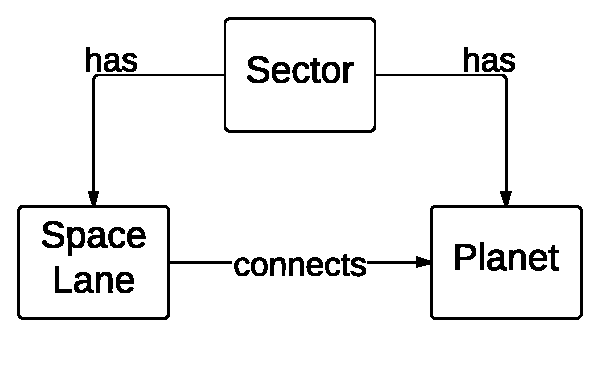
\includegraphics{res/model/sector.pdf}
% 	\caption{relationship between setor, planet, and space lanes}
% 	\label{fig:model:sectorRelation}
% \end{marginfigure}

\begin{margintable}
    \begin{tabular}{p{4em} p{11em}}
    \toprule
    \emph{Field} & \emph{Description} \\
    \midrule
    Name & Planet name \\
    Ecotype & Type of planet, e.g. star, ocean, or desert \\
    Location & Location of planet within the sector \\
    Resources & Quantity of resources generated by the planet if captured \\
    Capture status & Current owner of the planet, if any, and by how much they have captured it \\
    \bottomrule
    \end{tabular}
    \vspace{1em}
    \caption{Fields of the Planet model}
    \label{tab:planet-fields}
\end{margintable}

The list of planets that make up the sector are specified using the planetary model. Planets are modelled in such a way as to have a number of different fields that make the planet unique. Table~\ref{tab:planet-fields} gives a breakdown of the properties that comprise the model of a planet. Just like sectors, planets have a nickname to allow players to easily reference a specific planet instead of having to use location information or numerical identifiers. One of the most interesting pieces of the planetary model is the \emph{ecotype}. The ecotype of a planet specifies the type of ecological system that the planet represents, for example the ocean ecotype is used for planets that are almost entirely covered by water. This ecotype has a big effect on the planet because it determines the quantities of the different resources found in the planet.\sidenote{The use of resources is laid out in detail in Section~\ref{sec:resources}} This is because, for example, some ecotypes will have a greater proportion of metal (e.g.\ the metal ecotype). However, the quantity of resources stored by a planet is actually represented by a separate field instead of being statically determined by the ecotype. This was done to make it possible to add some more variety to the different planets. For example, it could be possible to use a random number generator to set the quantities of resources in a planet within the range specified by its ecotype. Currently all resource quantities are specified statically, but this potential enhancement would add some variables to the battles to keep the game interesting for regular players.

% TODO fix margin diagrams, all appearing below the page (invisible)
% \begin{marginfigure}
% 	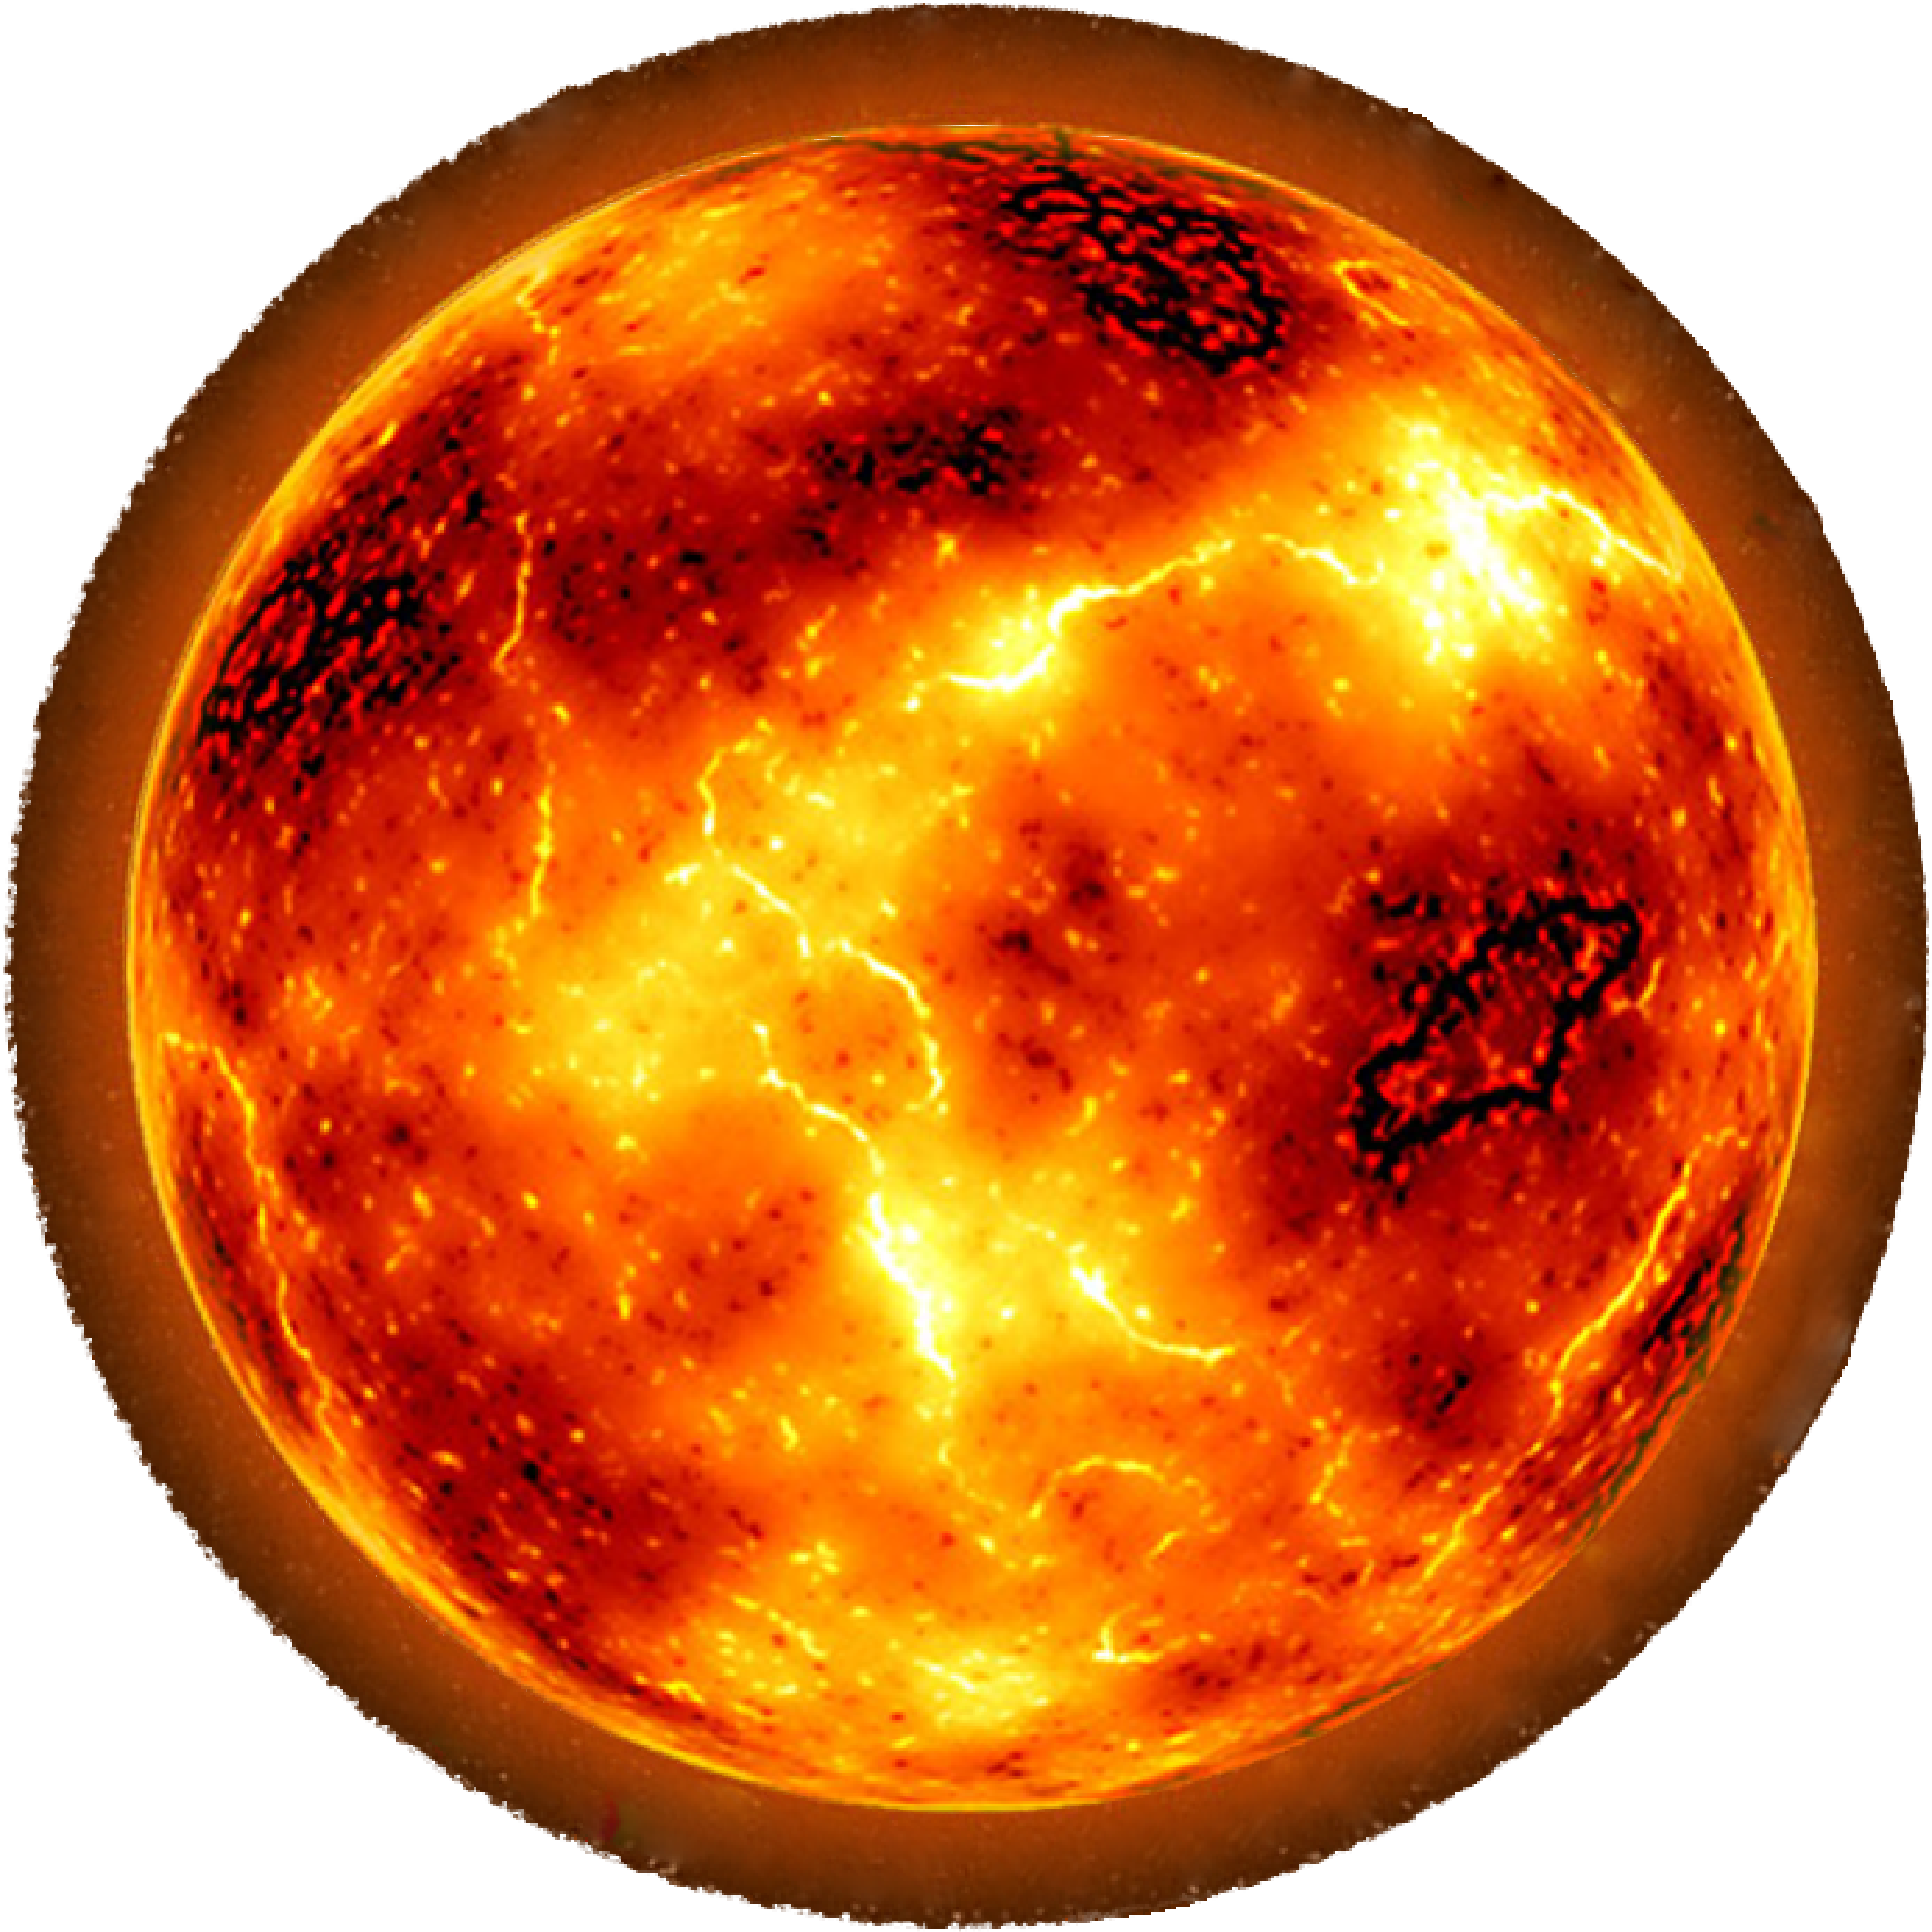
\includegraphics{res/planets/star.png}
% 	\caption{ecotype: star}
% 	\label{fig:model:starPlanet}
% \end{marginfigure}
% 
% \begin{marginfigure}
% 	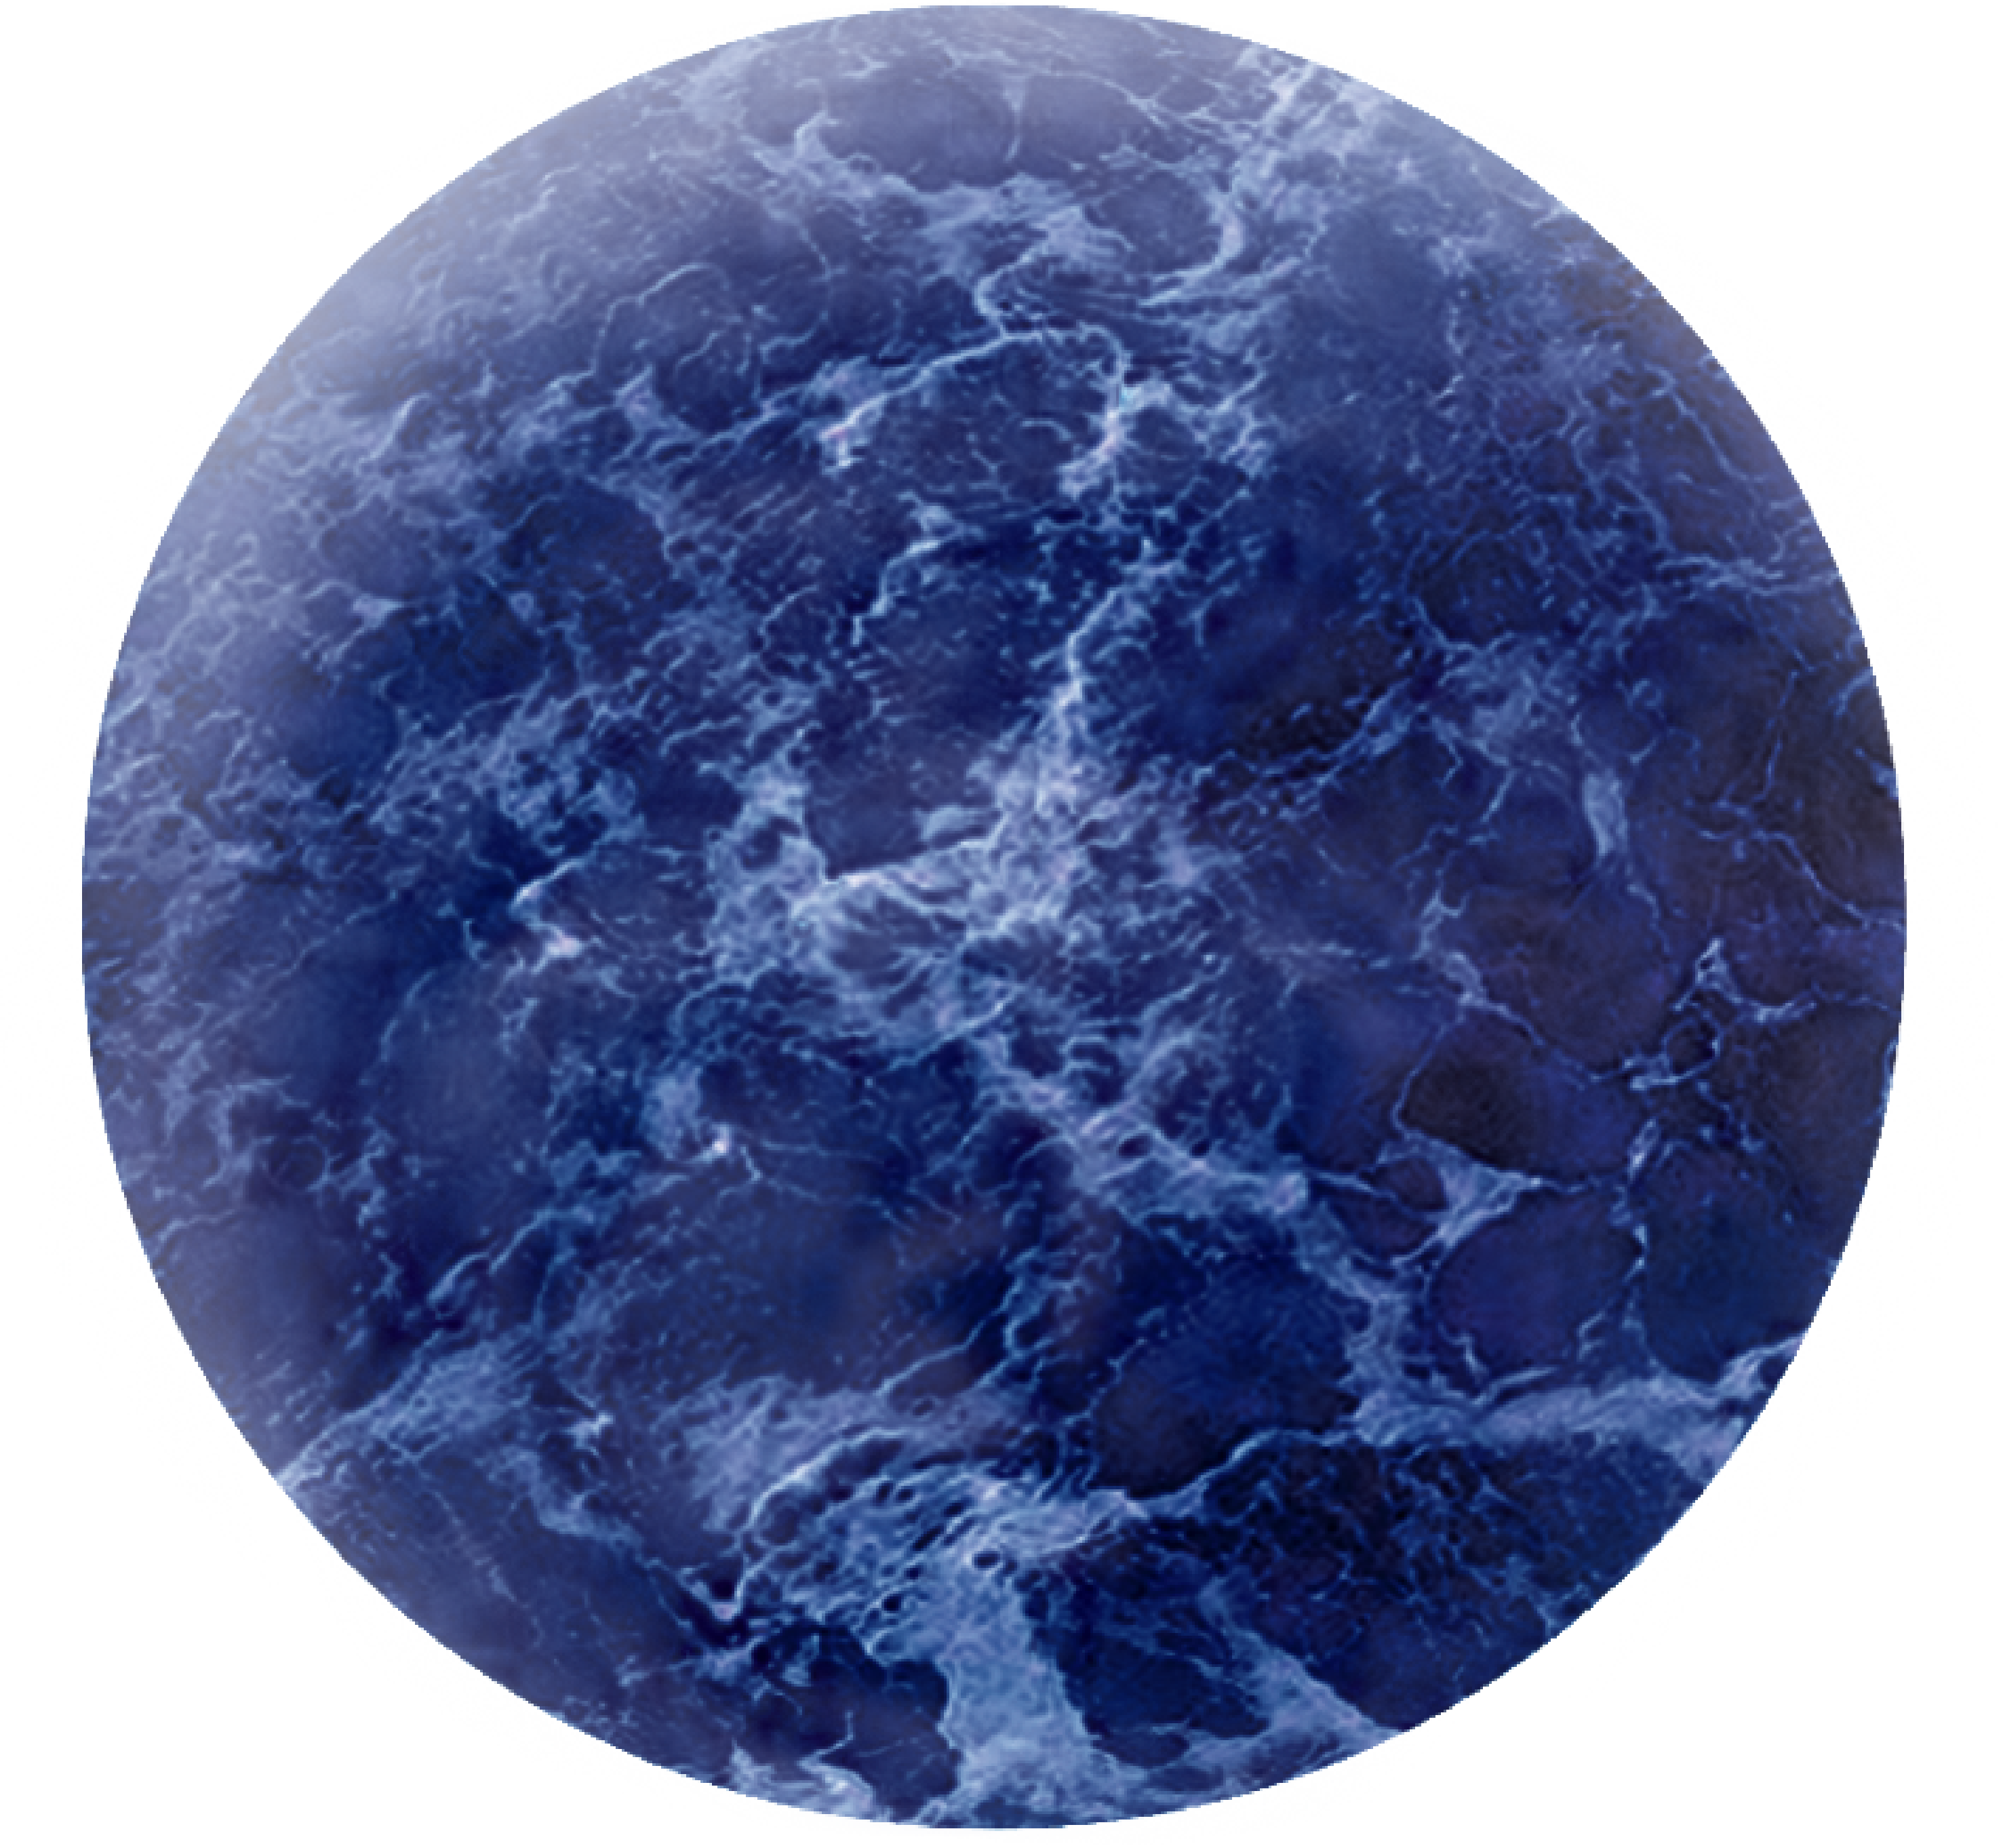
\includegraphics{res/planets/OceanPlanet.png}
% 	\caption{ecotype: ocean}
% 	\label{fig:model:oceanPlanet}
% \end{marginfigure}
% 
% \begin{marginfigure}
% 	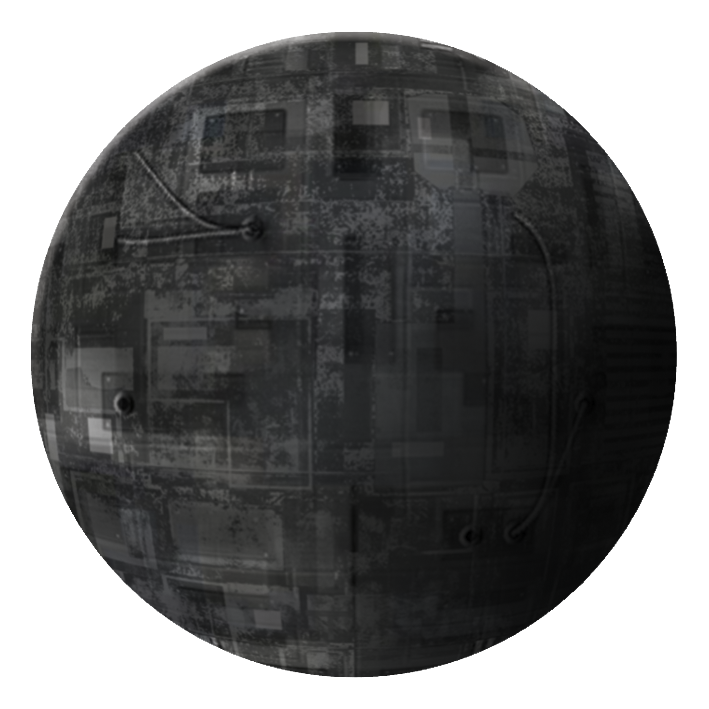
\includegraphics{res/planets/metal-planet.png}
% 	\caption{ecotype: metal}
% 	\label{fig:model:metalPlanet}
% \end{marginfigure}

\subsection{Ships, Classes and Configurations}

\begin{margintable}
    \begin{tabular}{p{4em} p{11em}}
    \toprule
    \emph{Field} & \emph{Description} \\
    \midrule
    Location & Current location of the ship within the sector \\
    Direction & The direction the ship is facing \\
    Damage & How much damage the ship has taken \\
    Order & Current player given order for the ship \\
    Goal & Current goal the ship is trying to achieve \\
    Plan & Current plan to execute in pursuit of the goal \\
    Targets & List of enemy ships that the ship is attacking \\
    Config. & Class of ship and its customisations \\
    \bottomrule
    \end{tabular}
    \vspace{1em}
    \caption{Fields of the Ship model}
    \label{tab:ship-fields}
\end{margintable}

The second set of models deals with the fleets of ships that are controlled by each player. A fleet is simply a list of ships which a client sends to the server having chosen which ships to include and made their customisations to these ships. The representation of a ship is actually broken down into a generic ship model and its specific configuration. The general ship model contains the configuration as well as the attributes that are updated during game play, such as the ship's orders and plans, and its current location and direction. The full list of fields for this model is shown in Table~\ref{tab:ship-fields}. The use of location, direction, and damage should hopefully be obvious. They are updated every tick by the server's main loop as the ship moves around the sector and engages with the enemy. Orders, goals, and plans are used by the artificial intelligence that controls the ships, see Section~\ref{sec:ai} for more details. The list of targets that a ship is currently attacking is also controlled by the artificial intelligence. The most interesting part of the ship is its configuration which specifies what base type the ship as and the customisations that have been applied by the user to this base.

The ship configuration contains the chosen ship class along with the lists of weapons and support systems that the player selected to add to the ship. The ship class represents the type of ship specifying the basic statistics of the ship. The set of statistics defined by the class is: ship speed, ship hull health, shield health, details of each of the weapon slots, details of the support system slots, and the cost of the ship. These statistics are used by the simulation code in the server to determine how the ship moves, how much more damage it can sustain before being destroyed, how much damage it does to the enemy ships it is attacking, and so on. A player is able to select the set of classes that they wish to include in their fleet, but they are restricted by a fixed budget. There are three ship classes that come with the game by default: corvette, destroyer, and dreadnought. The corvette is the smallest and quickest ship that can only be given one weapon. The destroyer is of middling strength and speed, it allows for five weapons to be added. Finally, the dreadnought is the largest and slowest of the three, but it packs the largest punch by supporting up to nine weapons.

This layered model approach to representing the ships was used to separate the different types of data that have to be stored. The ship model deals with the dynamic data that is updated during gameplay, the ship class is concerned with the static statistics that define the ships behaviour, and the configuration stores the user's customisations. This is useful because it allows a more efficient method of storing custom fleets on disk. Only the list of ship configurations needs to be kept since the class data is the same for all ships of the same type so can be loaded at run time and the rest of the ship data is only relevant during a battle.

% \begin{marginfigure}
% 	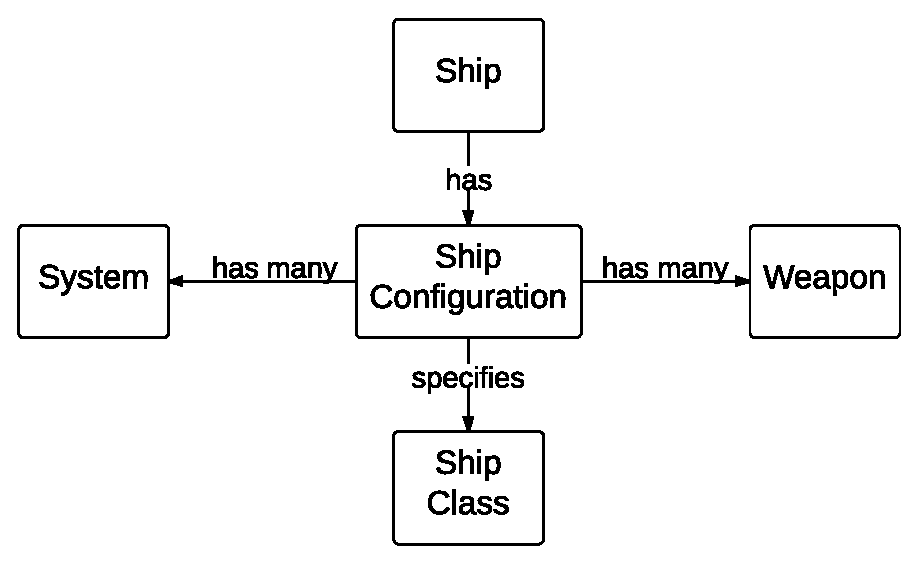
\includegraphics{res/model/ship.pdf}
% 	\caption{ship layout}
% 	\label{fig:model:shipRelation}
% \end{marginfigure}

\subsection{Weapons and Support Systems}

Talk about weapon types and systems.

\subsection{Defining Model Instances}

Talk about YAML configuration.
